\chapter{Introduction}
\label{chap:intro}


\section{Introduction to High Intensity Focused Ultrasound (HIFU)}

When one thinks of tumor surgery the things that come to mind are an operative room, lots of instruments to incise the body with surgeons holding them and finally a long recovery time where the affected patient has  to stay in special care for weeks, months or may be more. Such a treatment causes pre operative fear in patient's mind~\cite{Ramsay.1972.A.396}. Such pre-operative fear can in turns results in long recovery time, negative emotions and in some cases it forces the patient to use analgesics ~\cite{Sime1976}. These factors inspires people to develop an ideal tumor surgery which will avoid the above complications. An ideal tumor surgery would be a treatment which would require no incision and as a result shorter recovery time of the patient can be achieved This should be able to remove the affected tissue without damaging the adjacent structures near that tissue ~\cite{Jolesz...1}. The non-invasive nature of the treatment would be able change existing clinical practises and make it more patient friendly.

Magnetic resonance guided high intensity focused ultrasound treatment(MRgFUS) is considered to be a potential candidate for such an ideal tumor surgery ~\cite{Jolesz...1}. In this treatment Magnetic resonance imaging (MRI) is used to localized the target tumor. Then an ultrasound energy is generated by vibrating a piezoelectric materials and focused on the target tumor tissue (Figure~\ref{fig:Ultrasounf_focused}). The acoustic energy because of its unique nature just focused at the particular tumor tissue. Upon focusing the acoustic energy is converted into heat and thus thermally coagulate the tissue. The energy deposition doesn't cause any bio-effects to the adjacent healthy tissues or even tissues and skin on its path to the tumor tissue. The thermal ablation process require controlled monitoring in order to prevent overheating of tissues. MRI also has capability of mapping temporal and spatial distribution of tissues. This MRI feature is utilized to monitor the thermal ablation process..

\begin{figure}[t]
\centering
	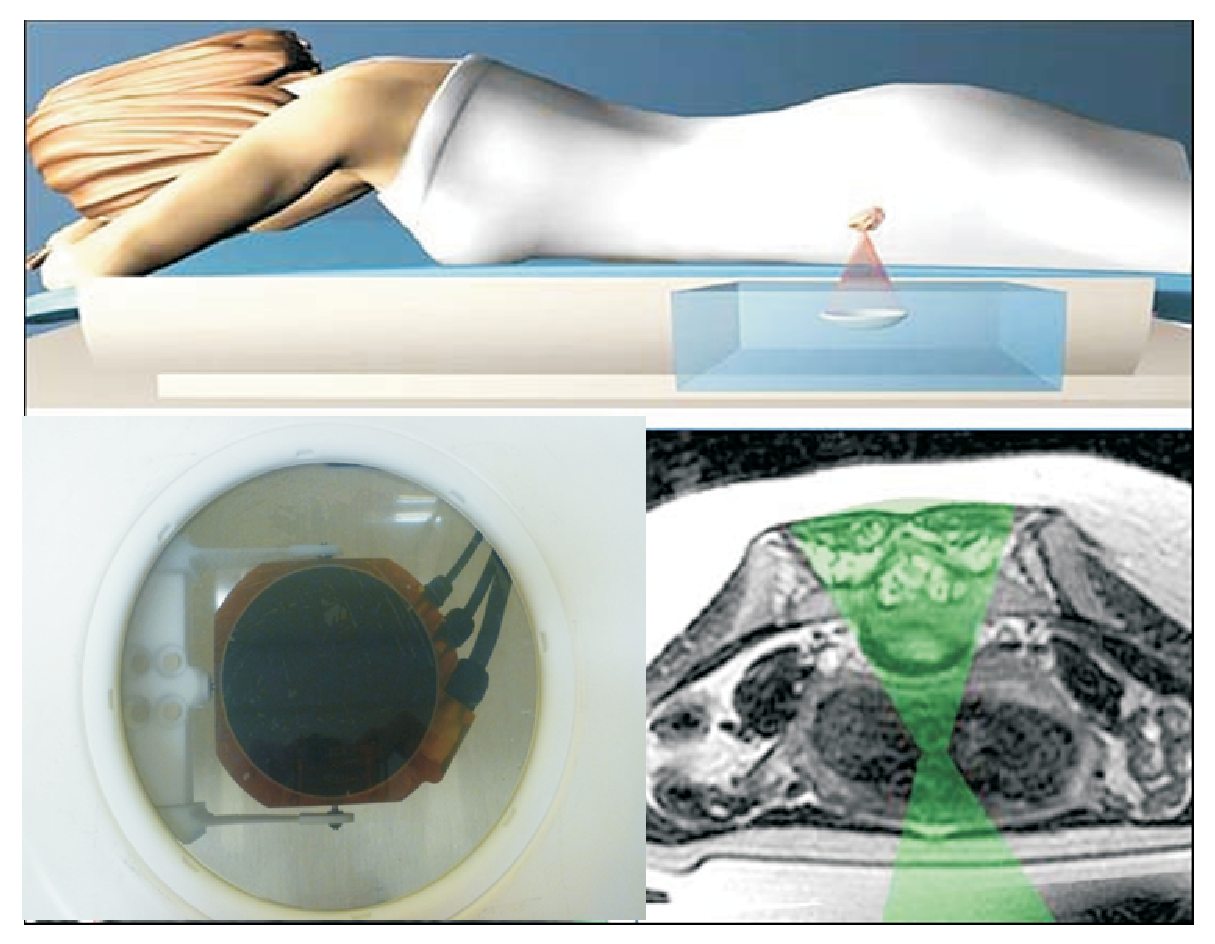
\includegraphics[width=0.7\textwidth]{Ultrasounf_focused.eps}\\
	\caption[Focusing of ultrasound]{Focusing of ultrasound\footnote}\label{fig:Ultrasounf_focused}

\end{figure}
\footnotetext{http://brainchemist.wordpress.com/2010/11/09/mri-guided-focused-ultrasound-surgery-radiology-brigham-and-womens-hospital-harvard}


\section{Basic Principle}
\subsection{Ultrasound Generation}
Ultrasound are basically sound waves with frequency greater than 1MHz. As human ear audible range is 20 Hz to 20000 KHz, it can't be heard by human being.Unlike other sound wave ultrasound propagate in a medium through vibration of molecules.First sound is generated from a source which initiate vibration. The vibration is transferred inside the medium to neighboring molecules. As a result compression and rarefaction takes place(Figure~\ref{fig:Compression and rarefaction}) where compression refers to the situation when molecules are pressed together or forced and rarefaction refers to the situation when the molecules are weakly bound or free to move.Moleculer vibration can take place in both longitudinal (longitudinal wave) and transverse(shear wave) direction. For medical ultrasound purposes shear wave is not used as it gets attenuated quickly is soft tissues~\cite{Hynynen...5,Carson.1978.JCU.126,Hunt.1987..354,Hynynen.1990..61}.


\begin{figure}[t]
\centering
	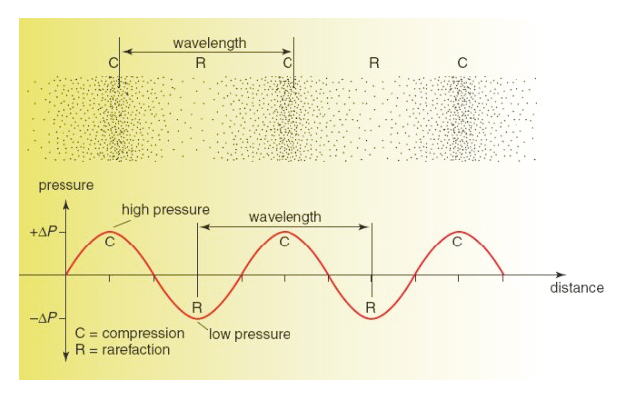
\includegraphics[width=0.7\textwidth]{Compressionandrarefactioncollected.eps}\\
	\caption[Compression and rarefaction of sound wave]{Compression and rarefaction of sound wave\footnote}\label{fig:Compression and rarefaction}
\end{figure}
\footnotetext{http://www.genesis.net.au/~ajs/projects/medical\_physics/ultrasound/index.html}

\subsection{Ultrasound Transducer}
Transducer is a device that converts one form of energy into another.Ultrasonic transducer is also one form of energy conversion device which converts electrical energy into mechanical energy using the piezoelectric effect.The transducer is operated at the resonance frequency of the piezoelectric material where it present higher response~\cite{Takasaki.2007..3817}.The piezoelectric materials vibrates with the cycles of contraction and expansion in response to the electrical energy by means of alternating current. As a result compression wave and expansion wave is generated.Possible dampening of the sound wave might occurs in situation where during cycles of contraction and expansion, expansion wave generated is weakened by an expansion wave. This represents a situation where compression wave is generated in one side of the materials before the expansion wave from other side has left the material. In a similar way, compression wave can also be weakened by expansion wave to dampen crystal response. In order to avoid these situations  careful control of the thickness of the piezoelectric materials according to the resonance frequency of the particular material. The established relationship between resonance frequency  and the thickness is 
 \begin{equation}\label{Eq:Phase-parallel}
    t=\frac{n\lambda}{2}
\end{equation}
Here \lambda is the wavelength of applied frequency and t is the effective thickness.
If this relationship is maintained the compression or expansion wave when it reaches the end of the material is aided constructively by another compression or expansion wave and thus amplifies the ultrasound wave.

Figure ~\ref{~fig:Ultrasound transducer} depicts a typical configuration of an ultrasound transducer. It is consists\cite{Hendee.2003..317}



\begin{figure}[t]
\centering
	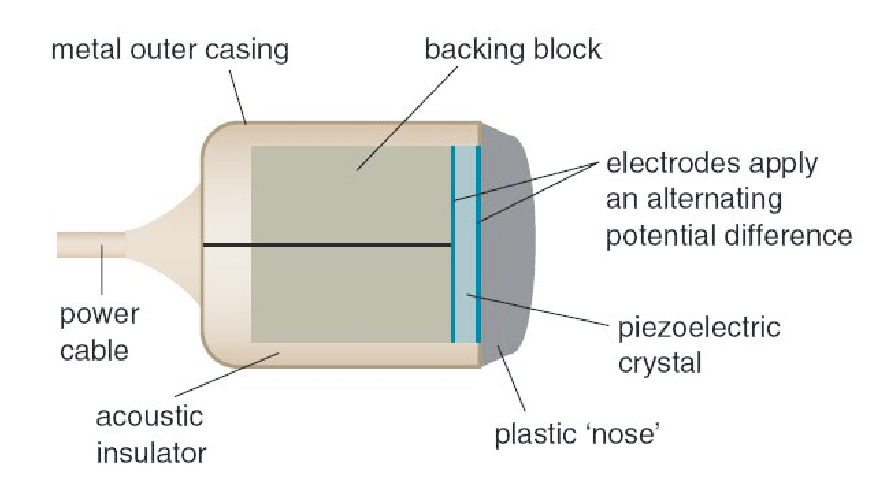
\includegraphics[width=0.7\textwidth]{UltrasoundTransducercollected.eps}\\
	\caption[Schematics of Ultrasound Transducer ]{Schematics of Ultrasound Transducer \footnote}\label{fig:Ultrasound transducer}
\end{figure}
\footnotetext{http://www.genesis.net.au/~ajs/projects/medical\_physics/ultrasound/index.html}


\section{Factor to focus:Dielectric dissipation factor, Hysteresis}
\section{Ferroelctricity}
\section{Formation of Perovskite based ferroelectric}

